\chapter{SPARSE MATRIX COMPRESSION}
\label{chp:compression}

Although we address this pillar last we view it as the most important. We previously implemented matrix compression in \cite{prelim:townsend}. However, we made the mistake of combining the two types of compression, index and floating point into one scheme. This simplified some aspects of the design. For example, this compression only needed to keep track of one data stream. Combining the two parts also makes sense if the two are correlated. In the extreme case the values in matrix could be calculated from the indices. However, we do not see an easy way to use this for general sparse matrix compression.

This chapter is dedicated to sprase pattern matrix compression, which we call SMC. In the next chapter we disscuss our floating point compression, which we call fzip. This chapter starts with Section~\ref{sec:index_compression_related_work} discussing related work. Then, Section~\ref{sec:index_compression_analysis} discusses the analysis of delta compression. Then, Section~\ref{sec:smc} discusses our implementation. Then, Section~\ref{sec:smc_decoder} discusses the hardware decorder for SMC. Lastly, Section~\ref{sec:smc_discussion} discusses something.

\section{Related Work}
\label{sec:index_compression_related_work}
Some work exists on compressing indices beyond coordinate (COO) format. The most obvious one and the one mentioned back in Chapter~\ref{chp:background} is compressed sparse row (CSR) format. The majority of work on computing SpMV on FPGAs uses CSR [\cite{prelim:nagar1}]. However we did find one alternative that uses a format called CVBV [\cite{prelim:kestur}]. Also, \cite{prelim:kourtis} uses index compression to speed up their CPU implementation. In addition to these we also look at how well gzip can compress indices.

Since both CVBV and the CPU method benefit from our RCR traversal we use that when analyzing them rather than row major traversal.
\subsection{CVBV}

Compressed Variable Bit Vector (CVBV) is a format created by [\cite{prelim:kestur}]. This implementation has two streams, which we will call the code stream and the argument stream. The code stream stores one 4 bit code for each delta. The first bit indicates what the type of the code is, dense (1) or regular (0). If the bit equals 1 (a dense code type) then the delta equals 1 and the value in the argument indicates how many deltas equal to 1 follow. If the bit equals 0 (a regular code type) then the delta equals the value in the argument.

The other 3 bits indicate how many nibbles are in the argument. The argument is taken from the argument stream. The results of this implementation is in Table~\ref{tbl:index} column 4.
\subsection{CPU method}

The method in [\cite{prelim:kourtis}] is similar but targeted for CPUs rather than FPGAs. Again there are 2 streams a code stream and an argument stream. The codes are 2 bytes long. Instead of one code per delta there is one code per array of deltas. The first byte indicates what size the deltas are, 1, 2, 4, or 8 bytes, and in the array is the last one in the row. The second byte indicates the length of the array.

The argument stream can be padded to make sure the data types align properly. The whole propose of this implementation is that nat\"ive data types are used so the CPU can process them faster. The compression results of this implementation is in Table~\ref{tbl:index} column 5.

\subsection{gzip}
We also choose to use the general compression program gzip in the comparison as well. Table~\ref{tbl:index} shows the compression of gzip on top of the CSR format. gzip does very well, partly because column indicies ofeten repeat.


\begin{table*}
\centering
\begin{threeparttable}
    \caption[Detailed analysis of index compression.]{This table shows the number of bytes per non-zero value the given index compression scheme achieves. (No floating point values are being compressed here.)}
\label{tbl:index}
\begin{tabular}{cccccccc}
\hline
\bfseries Matrix & \bfseries \tikz \node[rotate=90]{COO}; & \bfseries \tikz \node[rotate=90]{CSR}; & \bfseries \tikz \node[rotate=90]{CSR.gz}; & \bfseries \tikz \node[rotate=90]{cvbv}; & \bfseries \tikz \node[rotate=90]{cpu}; & \bfseries \tikz \node[rotate=90]{smc}; & \bfseries \tikz \node [rotate=90]{smc.gz};  \\
\hline
cant & 8.00 & 4.06 & 0.40 & 0.51 & 1.01 & 0.26 & 0.04 \\
consph & 8.00 & 4.06 & 0.19 & 0.45 & 1.01 & 0.26 & 0.03 \\
cop20k\_A & 8.00 & 4.18 & 1.07 & 0.99 & 1.01 & 0.64 & 0.54 \\
dense2 & 8.00 & 4.00 & 0.03 & 0.00 & 1.01 & 0.13 & 0.00 \\
mac\_econ\_fwd500 & 8.00 & 4.65 & 1.48 & 1.32 & 1.01 & 0.91 & 0.48 \\
mc2depi & 8.00 & 5.00 & 1.78 & 1.12 & 1.01 & 0.41 & 0.02 \\
pdb1HYS & 8.00 & 4.03 & 0.14 & 0.24 & 1.01 & 0.20 & 0.07 \\
pwtk & 8.00 & 4.07 & 0.16 & 0.23 & 1.01 & 0.19 & 0.01 \\
qcd5\_4 & 8.00 & 4.10 & 0.31 & 0.62 & 1.01 & 0.28 & 0.01 \\
rail4284 & 8.00 & 4.00 & 1.41 & 0.62 & 1.01 & 0.50 & 0.45 \\
rma10 & 8.00 & 4.08 & 0.20 & 0.38 & 1.01 & 0.24 & 0.09 \\
scircuit & 8.00 & 4.71 & 1.61 & 1.11 & 1.01 & 0.76 & 0.61 \\
shipsec1 & 8.00 & 4.07 & 0.20 & 0.45 & 1.01 & 0.22 & 0.06 \\
webbase-1M & 8.00 & 5.29 & 1.35 & 1.09 & 1.01 & 0.58 & 0.31 \\
\hline
average\tnote{a} & 8.00 & 4.33 & 0.79 & 0.70 & 1.01 & 0.42 & 0.21\\

\hline
\end{tabular}
\begin{tablenotes}
\item [a] Excludes the dense matrix.
\end{tablenotes}
\end{threeparttable}
\end{table*}

\section{Analysis}
\label{sec:index_compression_analysis}

We did some analysis on the distribution of deltas to come up with our implementation. The most important analysis was the distribution of delta lengths Table~\ref{tbl:index}. This table show the distribution of deltas for the RCR traversal. In this case we set the subwidth to 8 and the subheight to 512. There are some key characteristics to notice. First, about half of the deltas equal 1. Second, on average less than 5\% of the deltas are more than 512. Third, with some eye squinting the frequency distribution of the deltas is approximately a decreasing exponential.

\begin{sidewaystable}
\centering
\begin{threeparttable}
    \caption[The distribution of deltas by bit length.]{The distribution of the bit lengths required to store the delta length when using RCR traversal with the subheight set to 512 and the subwidth set to 8.}
\label{tbl:indexDist}
\begin{tabular}{cccccccccccc}
\hline
\bfseries Matrix & \bfseries 1 & \bfseries 2 & \bfseries 3-4 & \bfseries 5-8 & \bfseries 9-16 & \bfseries 17-32 & \bfseries 33-64 &\bfseries 65-128 & \bfseries 129-256 & \bfseries 257-512 & \bfseries 512+\\
\hline
cant & 72.2\% & 6.3\% & 6.8\% & 12.3\% & 0.7\% & 0.0\% & 0.0\% & 1.0\% & 0.0\% & 0.0\% & 0.6\% \\
consph & 76.6\% & 3.1\% & 5.9\% & 11.6\% & 0.8\% & 0.0\% & 0.0\% & 0.0\% & 0.1\% & 1.0\% & 0.8\% \\
cop20k\_A & 51.1\% & 1.9\% & 3.2\% & 22.9\% & 2.4\% & 1.0\% & 1.0\% & 1.0\% & 0.8\% & 0.7\% & 14.0\% \\
dense2 & 100.0\% & 0.0\% & 0.0\% & 0.0\% & 0.0\% & 0.0\% & 0.0\% & 0.0\% & 0.0\% & 0.0\% & 0.0\% \\
mac\_econ\_fwd500 & 8.2\% & 7.8\% & 7.3\% & 19.0\% & 12.0\% & 15.2\% & 6.3\% & 5.1\% & 2.8\% & 7.1\% & 9.2\% \\
mc2depi & 21.8\% & 0.0\% & 0.0\% & 24.9\% & 43.8\% & 0.0\% & 0.0\% & 0.0\% & 0.0\% & 0.1\% & 9.4\% \\
pdb1HYS & 88.0\% & 1.1\% & 3.6\% & 5.9\% & 0.0\% & 0.3\% & 0.2\% & 0.2\% & 0.1\% & 0.1\% & 0.4\% \\
pwtk & 87.7\% & 2.7\% & 3.0\% & 5.8\% & 0.0\% & 0.0\% & 0.0\% & 0.0\% & 0.0\% & 0.0\% & 0.8\% \\
qcd5\_4 & 66.0\% & 0.0\% & 8.2\% & 19.7\% & 3.6\% & 0.0\% & 0.0\% & 0.2\% & 0.0\% & 0.2\% & 2.1\% \\
rail4284 & 71.2\% & 1.0\% & 1.5\% & 5.3\% & 0.4\% & 1.0\% & 1.5\% & 1.5\% & 1.6\% & 2.0\% & 12.9\% \\
rma10 & 80.6\% & 1.4\% & 6.5\% & 8.8\% & 0.2\% & 0.8\% & 0.3\% & 0.1\% & 0.1\% & 0.2\% & 0.9\% \\
scircuit & 35.3\% & 2.8\% & 3.2\% & 25.7\% & 8.0\% & 3.5\% & 2.7\% & 2.3\% & 1.6\% & 1.1\% & 13.7\% \\
shipsec1 & 78.4\% & 0.0\% & 6.1\% & 12.2\% & 1.1\% & 0.0\% & 0.3\% & 0.2\% & 0.3\% & 0.2\% & 1.3\% \\
webbase-1M & 14.6\% & 3.5\% & 2.3\% & 37.7\% & 28.7\% & 1.0\% & 0.8\% & 0.5\% & 0.4\% & 0.4\% & 10.1\% \\
\hline
average\tnote{a} & 57.8\% & 2.4\% & 4.4\% & 16.3\% & 7.8\% & 1.8\% & 1.0\% & 0.9\% & 0.6\% & 1.0\% & 5.9\% \\
\hline
\end{tabular}
\begin{tablenotes}
\item [a] Excludes dense matrix
\end{tablenotes}
\end{threeparttable}
\end{sidewaystable}%

\section{Sparse Pattern Matrix Compression (SMC)}
\label{sec:smc}
We approach the problem of how to encode the series of deltas by giving each delta a code. We also created a special new line code. However, there are too many delta lengths to give each one a unique code. So we have 3 types of codes:
\begin{enumerate}
    \item Constant offset code.
    \item Variable offset code.
    \item New line code.
\end{enumerate}

The constant offset codes represent small deltas and decode as the exact value of the delta. The valiable offset codes represent larger deltas and decode as the bit length of the delta ($\textrm{log}_2(\delta)$). The new line codes represent the end of the 512 row section. After a newline code is read the running `major' row index will increment and the running `minor' row index will reset to -1 and all of the running column index will reset to -1.

Based on the analysis in Table~\ref{tbl:indexDist} we choose to have 32 constant offset codes. Using the deltas we can determine the frquencies of each code. With these frequencies we can create the codes using Huffman encoding [\cite{prelim:huffman}].

As an example, consider the example matrix back in Chapter~\ref{chp:background} in Equation~\ref{eqn:example}. Using row-major traversal (rather than RCR traversal) the deltas are:\\
1, 3, 3, \textbackslash n, 5, 3, \textbackslash n, 2, 1, 3, 1, \textbackslash n, 1, 4, \textbackslash n, 3, 1, 3, 1, \textbackslash n, 2, 3, \textbackslash n, 2, 1, 3, 2, \textbackslash n, 3, 1, 1, 1

Using 2 (rather than 32) constant offsets, the codes and their frequencies are:\\
\begin{enumerate}
    \item 1 : 10
    \item 2 : 4
    \item 3-4 : 9
    \item 5-8 : 1
    \item \textbackslash n : 7
\end{enumerate}
This results in 5 codes: 2 constant offset codes, 2 variable offsets codes, and 1 newline code. Now these codes are given varible length codes through Huffman encoding.

Huffman encoding first creates a huffman tree, which then is used to create the codes. The tree is created as follows. First, create a lone node for each code. Second, sort the nodes by frequency. Third, pop the two nodes with the lowest frequency from the list, and make the two nodes children of a new node. Fourth, set the frequency value of this new node to the sum of the frquencies of the children. Fifth, insert the new node back into the sorted list. Then repeat the third through fifth steps until the list only contains one node. \figurename~\ref{fig:huffman_tree} shows the creation of the Huffman tree. The following is the sorted list at each iteration:
\begin{enumerate}
    \item (1 : 10), (3-4 : 9), (\textbackslash n : 7), (2 : 4), (5-8 : 1)
    \item (1 : 10), (3-4 : 9), (\textbackslash n : 7), (a : 5)
    \item (b : 12), (1 : 10), (3-4 : 9)
    \item (c : 19), (b : 12)
    \item (d : 31)
\end{enumerate}
\begin{figure}
    \begin{subfigure}{.2\linewidth}
        \centering
        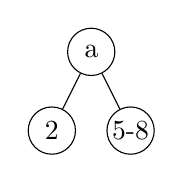
\begin{tikzpicture}
            \node(a)[circle,draw,inner sep=0pt,minimum size=.6cm] at (0,0){a};
            \node(2)[circle,draw,inner sep=0pt,minimum size=.6cm] at (-.5,-1){2};
            \node(58)[circle,draw,inner sep=0pt,minimum size=.6cm] at (.5,-1){5-8};
            \draw (a) -- (2);
            \draw (a) -- (58);
        \end{tikzpicture}
        \caption{Added `a'}
        \label{fig:Huffmantree1}
    \end{subfigure}
    \begin{subfigure}{.2\linewidth}
        \centering
        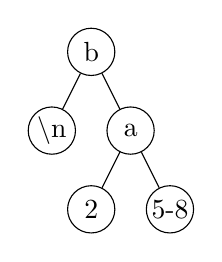
\begin{tikzpicture}
            \node(n)[circle,draw,inner sep=0pt,minimum size=.6cm] at (-1,0){\textbackslash n};
            \node(b)[circle,draw,inner sep=0pt,minimum size=.6cm] at (-.5,1){b};
            \node(a)[circle,draw,inner sep=0pt,minimum size=.6cm] at (0,0){a};
            \node(2)[circle,draw,inner sep=0pt,minimum size=.6cm] at (-.5,-1){2};
            \node(58)[circle,draw,inner sep=0pt,minimum size=.6cm] at (.5,-1){5-8};
            \draw (a) -- (2);
            \draw (a) -- (58);
            \draw (b) -- (n);
            \draw (b) -- (a);
        \end{tikzpicture}
        \caption{Added `b'}
        \label{fig:Huffmantree2}
    \end{subfigure}
    \begin{subfigure}{.5\linewidth}
        \centering
        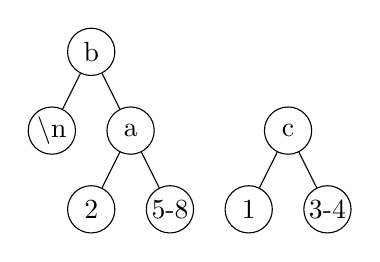
\begin{tikzpicture}
            \node(n)[circle,draw,inner sep=0pt,minimum size=.6cm] at (-1,0){\textbackslash n};
            \node(b)[circle,draw,inner sep=0pt,minimum size=.6cm] at (-.5,1){b};
            \node(a)[circle,draw,inner sep=0pt,minimum size=.6cm] at (0,0){a};
            \node(2)[circle,draw,inner sep=0pt,minimum size=.6cm] at (-.5,-1){2};
            \node(58)[circle,draw,inner sep=0pt,minimum size=.6cm] at (.5,-1){ 5-8 };
            \node(1)[circle,draw,inner sep=0pt,minimum size=.6cm] at (1.5,-1){ 1 };
            \node(34)[circle,draw,inner sep=0pt,minimum size=.6cm] at (2.5,-1){ 3-4 };
            \node(c)[circle,draw,inner sep=0pt,minimum size=.6cm] at (2,0){c};
            \draw (a) -- (2);
            \draw (a) -- (58);
            \draw (b) -- (n);
            \draw (b) -- (a);
            \draw (c) -- (1);
            \draw (c) -- (34);
        \end{tikzpicture}
        \caption{Added `c'}
        \label{fig:Huffmantree3}
    \end{subfigure}
    \begin{subfigure}{.45\linewidth}
        \centering
        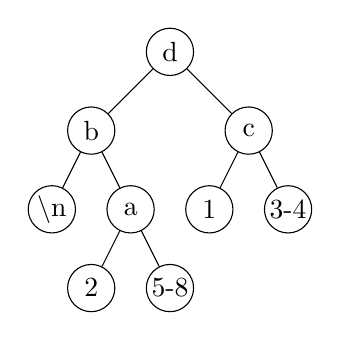
\begin{tikzpicture}
            \node(n)[circle,draw,inner sep=0pt,minimum size=.6cm] at (-1,0){\textbackslash n};
            \node(b)[circle,draw,inner sep=0pt,minimum size=.6cm] at (-.5,1){b};
            \node(a)[circle,draw,inner sep=0pt,minimum size=.6cm] at (0,0){a};
            \node(2)[circle,draw,inner sep=0pt,minimum size=.6cm] at (-.5,-1){2};
            \node(58)[circle,draw,inner sep=0pt,minimum size=.6cm] at (.5,-1){ 5-8 };
            \node(1)[circle,draw,inner sep=0pt,minimum size=.6cm] at (1,0){ 1 };
            \node(34)[circle,draw,inner sep=0pt,minimum size=.6cm] at (2,0){ 3-4 };
            \node(c)[circle,draw,inner sep=0pt,minimum size=.6cm] at (1.5,1){c};
            \node(d)[circle,draw,inner sep=0pt,minimum size=.6cm] at (.5,2){d};
            \draw (a) -- (2);
            \draw (a) -- (58);
            \draw (b) -- (n);
            \draw (b) -- (a);
            \draw (c) -- (1);
            \draw (c) -- (34);
            \draw (d) -- (b);
            \draw (d) -- (c);
        \end{tikzpicture}
        \caption{Added `d'}
        \label{fig:Huffmantree3}
    \end{subfigure}
    \caption{trees}
    \label{fig:huffman_tree}
\end{figure}

To encode a large delta with a variable length code, the delta (minus the most significant bit) is pushed onto an argument stream. In the end the SMC file has three parts: the header, the dictionary, the codes stream, and the argument stream.

To make decoding easier we set the maximum code length to 9. We do this by artificially increasing the frequency of each code to a minimum of $\frac{nnz}{2^9}$. In the SMC file a code dictionary needs to be present so that the file can be decompressed. For easier decoding we have $2^9$ records with all the information to decode them.

\section{The SMC decoder}
\label{sec:smc_decoder}
The hardware decoder relies on lookup tables to decode the two streams (see \figurename~\ref{fig:smc_decoder}). First the dictonary is loaded onto a large 512 value lookup table (LUT). This lookup table uses the code length to determine how much to right shift the first shift buffer. The LUT then determines if the second shift buffer is needed (the code is a variable length delta). In that case, the second shift buffer is right shifted and the output is used to create the delta. Then the delta (or newline) is sent to the running row and column index and the current row and column index is outputed from the decoder.
\begin{figure}
    \centering
    \begin{tikzpicture}
        \node at (0,1) {Memory};
        \node at (4,1) {Decoder};
        \draw [dashed](1.5,1.5) -- (1.5,-4);
        \node at (0,0)[draw,trapezium,trapezium right angle=120,trapezium left angle=60](h){Header};
        \node at (0,-1)[draw,trapezium,trapezium right angle=120,trapezium left angle=60](d){Dictionary};
        \node at (0,-2.2)[draw,trapezium,trapezium right angle=120,trapezium left angle=60](ds){\shortstack{Data\\Stream}};
        \node at (0,-3.6)[draw,trapezium,trapezium right angle=120,trapezium left angle=60](as){\shortstack{Argument\\Stream}};

        \node at (4, 0) [draw,minimum width=4cm](sb1){Shifter Buffer};
        \node at (2.5, -1.5) [draw,minimum height=1cm](l){LUT};
        \node at (4, -3) [draw,minimum width=4cm](sb2){Shifter Buffer};
        \node at (5.5, -1.5) [draw,minimum height=1cm](dti){\shortstack{Delta to\\Index}};
        \node at (7, -1)(r){row};
        \node at (7, -2)(c){col};

        \draw[->,shorten >=2pt] (ds) .. controls ++(1.5,0)  and ++(-2.5,0) .. (sb1);
        \draw[->,shorten >=2pt] (sb1.350) .. controls ++(0,-.5) and ++(0,.5) .. (l.north -| 2.6,0);
        \draw[<-,shorten <=2pt] (sb1.south -| 2.4,0) .. controls ++(0,-.5) and ++(0,.5) .. (l.north -| 2.3,0);
        \draw[->,shorten >=2pt] (as) .. controls ++(1.5,0) and ++(-2.5,0) .. (sb2);
        \draw[->,shorten >=2pt] (l) -- (l|-sb2.north);
        %\draw (l) |- (sb2);
        \draw[->,shorten >=2pt] (sb2.10) .. controls ++(0,.5) and ++(-1,0) .. (4,-1.5);
        \draw[->,shorten >=2pt] (d) .. controls ++(1.5,0) and ++(-1,0) .. (l);
        \draw[->,shorten >=2pt] (l) -- (dti);
        \draw[->,shorten >=2pt] (dti) -- (r);
        \draw[->,shorten >=2pt] (dti) -- (c);

    \end{tikzpicture}
    \caption{The hardware design of the SMC decoder.}
    \label{fig:smc_decoder}
\end{figure}

We do not have the exact area and performance of this decoder because we only designed a decoder that combined the index and floating point decoding. However, the first shift buffer uses 293 LUTs and 60 registers. The second shift buffer uses 469 LUTs and 82 registers. The combined decoder has a top frequency of 150 Mhz after place and route using xst.

\section{Results}
\label{sec:smc_discussion}

Table~\ref{tbl:index}  shows the results of SMC compression. As seen, it outperforms the pervious implementations. In addition, we looked at compressing the smc file further with gzip. This achieve a good deal of addition compression. One reason for this additional compression is that it compresses the repeating deltas equal to 1 in the dense sections of the matrix.
